% Pablo Baeyens (@pbaeyens)
% Email: pbaeyens31+github@gmail.com
% Licencia: CC BY-SA 3.0

%% Paquetes y configuración %

% Beamer
\PassOptionsToPackage{unicode}{hyperref}  % Evita errores con caracteres no ASCII
\PassOptionsToPackage{naturalnames}{hyperref} % tex.stackexchange.com/questions/10555
\documentclass[compress]{beamer}

% Idioma
\usepackage[spanish]{babel} % Traducciones
\usepackage[utf8]{inputenc} % Uso de caracteres UTF-8
\usepackage{lmodern}        % Fuentes de tamaño arbitrario
\usepackage[T1]{fontenc}    % Permite copiar y evita errores
\uselanguage{Spanish}       % Traducciones beamer
\languagepath{Spanish}      % (tex.stackexchange.com/questions/168208)

% Matemáticas
\usepackage{amsfonts}
\usepackage{amsmath}
\usepackage{amssymb}

% Colores
\definecolor{backg}{HTML}{F2F2F2}    % Fondo
\definecolor{title}{HTML}{bdc3d1}    % Títulos
\definecolor{comments}{HTML}{BDBDBD} % Comentarios
\definecolor{keywords}{HTML}{08388c} % Palabras clave
\definecolor{strings}{HTML}{FA5858}  % Strings
\definecolor{links}{HTML}{2C2C95}    % Enlaces
\definecolor{bars}{HTML}{045FB4}     % Barras (gráfico)

% Código
\usepackage{listings}
\lstset{
language=[LaTeX]TeX,
basicstyle=\footnotesize,
morekeywords={href,uselanguage,languagepath,column},
otherkeywords={pause,usetheme,usecolortheme,useinnertheme,titlepage,tableofcontents,subtitle},
breaklines=true,
backgroundcolor=\color{backg},
keywordstyle=\color{keywords},
commentstyle=\color{comments},
stringstyle=\color{strings},
tabsize=2,
% Acentos, ñ, ¿, ¡ (tex.stackexchange.com/questions/24528)
extendedchars=true,
literate={á}{{\'a}}1 {é}{{\'e}}1 {í}{{\'i}}1 {ó}{{\'o}}1
         {ú}{{\'u}}1 {ñ}{{\~n}}1 {¡}{{\textexclamdown}}1
         {¿}{{?`}}1
}

% Gráficos
\usepackage{pgfplots}
\pgfplotsset{width=7cm,compat=1.8} % Opciones para gráficos

% Columnas
\usepackage{multicol}

% Emoticonos
\usepackage{wasysym}

% tikz
\usepackage{tikz}
\usetikzlibrary{mindmap,trees,shadows}
\tikzset{ % Genera overlays
    invisible/.style={opacity=0},
    visible on/.style={alt={#1{}{invisible}}},
    alt/.code args={<#1>#2#3}{\alt<#1>{\pgfkeysalso{#2}}{\pgfkeysalso{#3}}},
}
%\usepackage{gnuplot-lua-tikz}

%% Comandos %%
\newcommand{\ejemplo}[1]{\lstinputlisting{./examples/#1}} % Mostrar código de ejemplos
\newcommand{\muestra}[1]{\input{./examples/#1}}           % Mostrar ejemplos
\newcommand{\seccion}[1]{\input{./sections/#1}}           % Incluir secciones
\newcommand{\espacio}{\vspace*{\baselineskip}}            % Añade espacios
\newcommand{\beamer}{\texttt{beamer} }                    % Estilo único para beamer
\newcommand{\enlace}[3]{\href{#1}{\textbf{#2}} - {\small #3}}  % Estílo único para refs
\newcommand{\comando}[1]{{\color{black}\textbackslash}{\color{keywords}#1}}

%% Temas %%
% Tema y tema de color
  \usetheme{Malmoe}
  \usecolortheme{wolverine}
% \useinnertheme{circles}
  \setbeamercovered{transparent}
% Colores bloques
%  \setbeamercolor{block title}{bg=title,fg=links}
%  \setbeamercolor{block body}{bg=backg,fg=black}
%  \setbeamercolor{block title alerted}{fg=red!70!black,bg=title!92!red}
%  \setbeamercolor{block body alerted}{fg=black,bg=backg}
%  \setbeamercolor{block title example}{fg=green!70!black,bg=title!92!green}
%  \setbeamercolor{block body example}{fg=black,bg=backg}
% Enlaces (tex.stackexchange.com/questions/13423)
\hypersetup{colorlinks,linkcolor=,urlcolor=links}
% Quita enlaces de navegación (stackoverflow.com/questions/3017030)
\setbeamertemplate{navigation symbols}{}
% Quita barra inferior (stackoverflow.com/questions/1435837)
\setbeamertemplate{footline}{}
% Evita warnings boxes
\hfuzz=20pt
\vfuzz=20pt
% Evita wranings itemize
\renewcommand\textbullet{\ensuremath{\bullet}}
\definecolor{naranja}{RGB}{252,187,6}
\definecolor{verde}{RGB}{64,159,64}

% tikz
\usepackage{tikz}
\usepackage{ragged2e}
\usetikzlibrary{shapes.multipart}

\usepackage{color}


%% Título y otros %%
\title{Apache OFBiz} % Título
\subtitle{
Diseño y desarrollo de sistemas de información (2017-2018)\\
Doble Grado en Ingeniería Informática y Matemáticas
}                                  % Subtítulo
\date{\today} % Fecha


%%%%%%%%%%%%%%%%%%%%%%%%%%%%%%%%%%%%%%%%%%%%%%%%%%%%%%%%%%%%%%%%

%% Presentación %%
\begin{document}

\begin{frame}
\titlepage
\end{frame}

\begin{frame}{Índice}
  \hypertarget{index}{}
  \tableofcontents
\end{frame}

\section{Información}
\begin{frame}{Apache OFBiz}
Según la \href{https://cwiki.apache.org/confluence/display/OFBIZ/Philosophy}{wiki de la Apache Software Foundation}, Apache ofbiz es un ERP gratuito creado por la fundación apache.

	\begin{figure}[H]
	\centering
	
\includegraphics[width=0.4\linewidth]{img/1.png}
\end{figure}

El código del ERP lo matiene la comunidad.

Se fundó bajo 5 conceptos, las 5 E's.

\begin{enumerate}
	\item Ease of Cost
	\item Ease of Installation
	\item Ease of Customization
	\item Ease of Integration
	\item Ease of Use
\end{enumerate}

\end{frame}


\begin{frame}{Apache Software Foundation}

Según su propia \href{https://www.apache.org/foundation/}{página oficial}, es una entidad sin ánimo de lucro, reguladora de los proyectos de software relacionados con Apache, desde el servidor http hasta nuestro ERP.
\vspace{.5cm}

Dispone de una comunidad de más de 5,500 programadores que colaboran en mantener todos los proyectos de la fundación.

\begin{figure}[H]
	\centering
	
\includegraphics[width=0.5\linewidth]{img/2.png}
\end{figure}
\end{frame}

\section{Instalación}
\begin{frame}{Instalación de Apache Ofbiz}

	Apache Ofbiz necesita el 'java development kit' (jdk) descargable en la web: \href{http://www.oracle.com/technetwork/java/javase/downloads/jdk8-downloads-2133151.html}{http://www.oracle.com/technetwork/java/javase/downloads/jdk8-downloads-2133151.html}
	
	Después de la instalación del 'jdk' ejecutamos en el directorio principal del programa : ./gradlew cleanAll loadDefault
	
	Es posible que nos encontremos con un error en la variable JAVA\_HOME.
	\begin{figure}[H]
		\centering
		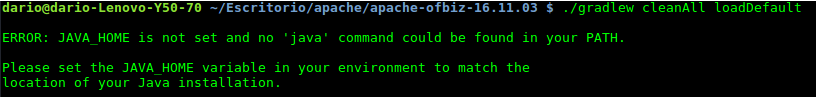
\includegraphics[width=1.0\linewidth]{img/3.png}
	\end{figure}

\end{frame}

\begin{frame}{Solucion del error en la variable JAVA\_HOME}
	Solución:
	\begin{enumerate}
		\item Descargar el archivo .tar.gz de jdk de la página anterior.
		\item Descomprimir y entrar en la carpeta.
		\item Ejecutar JAVA\_HOME=`pwd`, export JAVA\_HOME
		\item volver a la carpeta de Apache Ofbiz y volver a ejecutar ./gradlew cleanAll loadDefault
	\end{enumerate}

\end{frame}

\begin{frame}
Para iniciar el ERP ejecutamos ./gradlew ofbiz.

En la terminal veremos que se muestra una barra de progreso que no avanza del 91\%.
Llegados a este punto Apache ofbiz ya se puede ejecutar.

\begin{figure}[H]
	\centering
	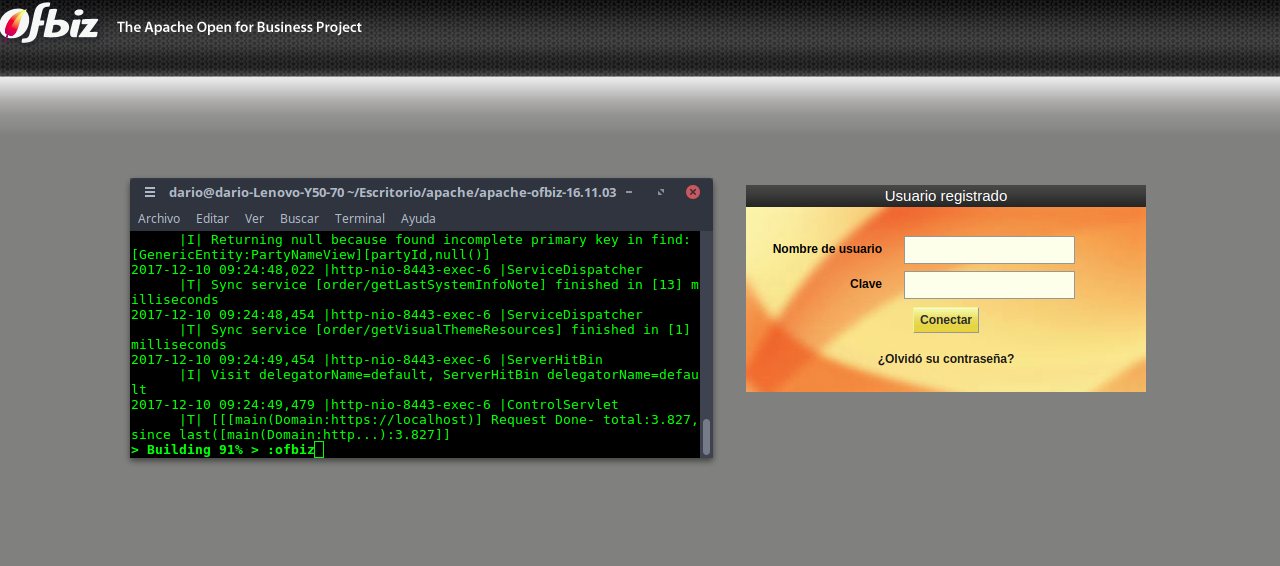
\includegraphics[width=0.65\linewidth]{img/4.png}
\end{figure}

Podemos acceder al ERP desde nuestro navegador:

[Order Back Office](https://localhost:8443/ordermgr)

[Accounting Back Office](https://localhost:8443/accounting)

[Administrator interface](https://localhost:8443/webtools)

La contraseña y el usuario son 'ofbiz' y 'admin' respectivamente, tal y como se explica en el README cuando lo descargamos.
\end{frame}



\section{Funcionalidades}
\subsection{Lista de funcionalidades}
\begin{frame}{Funcionalidades}
\begin{columns}[T]
	\begin{column}{.5\textwidth}
	\begin{itemize}
		\item Comercio electrónico
		\item Gestión de catálogo
		\item Gestión de precios y ofertas
		\item Gestión de usuarios
		\item Gestión de fabricación
		\item Gestión de encargos (compras y ventas)
		\item Gestión de contabilidad
		
	\end{itemize}
\end{column}
	\begin{column}{.5\textwidth}
	\begin{itemize}
		\justifying
		\item Empaquetado y envío
		\item Gestión de tareas, trabajos y proyectos
		\item Gestión de contenido (webs, blogs, foros o contenido general)
		\item Internacionalización y localización
	\end{itemize}
\end{column}
%Ref https://cwiki.apache.org/confluence/display/OFBIZ/OFBiz+Features#OFBizFeatures-BaseApplications
\end{columns}

\end{frame}

\begin{frame}
\begin{figure}[H]
	\centering
	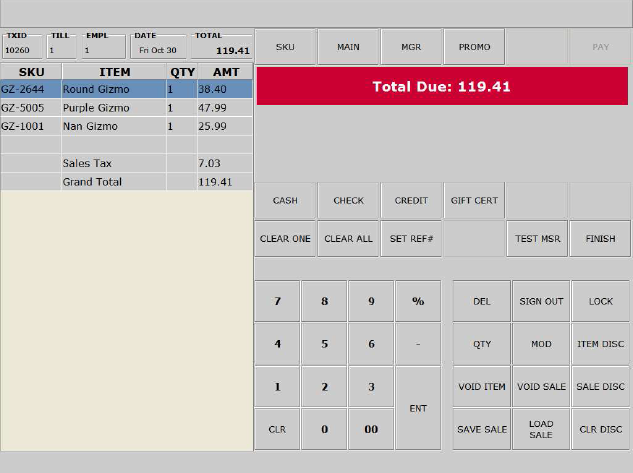
\includegraphics[width=0.9\linewidth]{img/posOfbiz.png}
	\caption{Captura de la funcionalidad Point Of Sales que ofrece Ofbiz, que es uno de los puntos más atractivos de este software}
	%Ref: https://cwiki.apache.org/confluence/display/OFBIZ/Information+on+translated+languages+in+OFBiz
\end{figure}

\end{frame}

\begin{frame}{Críticas a las funcionalidades}
\begin{columns}[T]
	
	\begin{column}{.5\textwidth}
		\justifying
		Algunas funcionalidades realmente necesarias, como la localización, están \textbf{incompletas}.
		\begin{figure}[H]
			\centering
			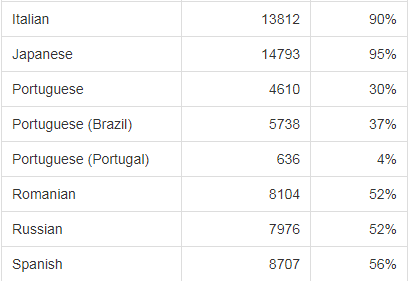
\includegraphics[width=0.8\linewidth, height=0.5\linewidth]{img/localisation.png}
			
		\end{figure}
		
		No hay funcionalidad para \textbf{contratación}, \textbf{tiempo de trabajo} ni \textbf{nómina}. 
	\end{column}
	\begin{column}{.5\textwidth}
		Faltan funcionalidades para \textbf{exportar} información, como por ejemplo PDFs o documentos de texto.
		\vspace{.5cm}
		
			
		\vspace{.5cm}
		
		Por último, no hay soporte directo para manejar el ERP desde \textbf{dispositivos móviles}, y se necesita software adicional para implementarlo.
	\end{column}
	
\end{columns}
	
\end{frame}



\section{Ventajas}
\begin{frame}{Ventajas y desventajas}
	\begin{columns}[T]
		\begin{column}{.5\textwidth}
			\textbf{Ventajas destacables:}
			\begin{itemize}
				\item Independiente de la base de datos.
				\item Tiene MMS (Software de Mantenimiento de la Gestión).
				\item Una vez configurado, se puede usar todo el primer día con facilidad.
				\item Tiene demo online.
			\end{itemize}
		\end{column}
		
		\begin{column}{.5\textwidth}
			\textbf{Desventajas:}
			\begin{itemize}
				\item Instalación poco pulida (no llega al 100\%).
				\item Complicado de configurar.
				\item Localización.
				\item No hay funcionalidad para contratación.
				\item Falta funcionalidad para exportar.
				\item No manejable por móvil.
			\end{itemize}
		\end{column}
	\end{columns}
\end{frame}



\section{Adopción}
\begin{frame}{Tendencias}
	\begin{figure}[H]
		\centering
		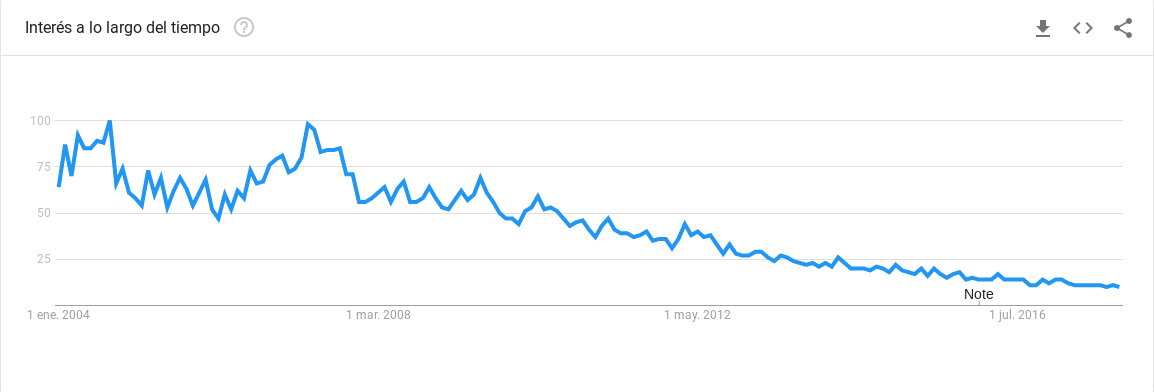
\includegraphics[width=1.0\linewidth]{img/tendencia_tiempo.png}
	\end{figure}
	\begin{figure}[H]
		\centering
		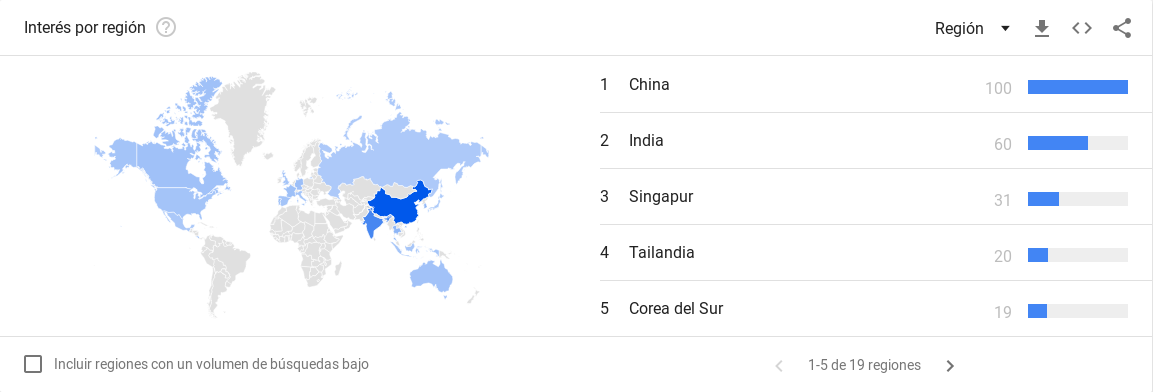
\includegraphics[width=1.0\linewidth]{img/tendencia_lugar.png}
	\end{figure}
\end{frame}

\begin{frame}{Algunas empresas que lo han implantado}
	OFBiz es utilizado mayoritariamente por empresas de comercio electrónico.\\

	\begin{block}{Ejemplos}
		\begin{itemize}
			\item \textbf{bebepeque.com} \\
				Tienda de articulos para bebés.
			\item \textbf{stchristopherpendants.com.uk} \\
				Tienda de colgantes especializada en joyería católica.
			\item \textbf{ww8.prathambooks.com} \\
				La mayor editorial de libros infantiles de India.
			\item \textbf{petsprite.com} \\
				Tienda de comida y equipamiento para mascotas.
		\end{itemize}
	\end{block}
\end{frame}

\begin{frame}{Casos de éxito}
	\begin{block}{borngifted.co.uk}
		\begin{quotation}
			``OFBiz has provided us with a \textbf{reliable and flexible}
			e-commerce solution with enhanced customer functionality e.g.
			customer product reviews, gift selector, special offers and cross
			selling capabilities. [...] the Customer Relationship Manager
			allows us to communicate effectively with our customers
			via email newsletters.''\\
		\end{quotation}
	\end{block}
	\begin{block}{graciousstyle.com}
		\begin{quotation} 
			``We've found that OFBiz is an extremely
			\textbf{advanced and flexible} platform that is
			\textbf{well-suited} to the ever-changing needs of a growing
			company. [...] there is a \textbf{strong development community}
			which is actively moving OFBiz forward.''
		\end{quotation}
	\end{block}
\end{frame}

\begin{frame}{Críticas}
	\begin{quotation}
		``To anybody considering OFBiz... I recommend you run away, screaming in
		terror, and get as far away from it as you can, and stay there.
		Seriously, looking at the code for OFBiz is like reading from the
		Necronomicon... it exposes you to horrors that mortal men were never
		meant to be exposed to. Read from the OFBizicom and your eyes will
		start bleeding black oil, your skin will break out with festering sores
		of malfeasance, and your dreams will be plagued by nightmare visions
		of death, devastation and destruction for all eternity.

		OTOH, if you REALLY like XML and think that XML is a good way
		to do everything under the sun, including defining the syntax for
		your own bizarro programming language... then jump right in.''\\
		- mindcrime -
	\end{quotation}
\end{frame}



\end{document}
